\section{含有四个味的 $\SU(2)$ 理论与 Gaiotto 对偶}\label{sec:gaiotto}\index{SU2FourFlavors@含四个味的 $\SU(2)$ 理论|hyperpage}\index{GaiottoDuality@Gaiotto 对偶|hyperpage}
本节从含有 $N_f=4$ 个味的 $\SU(2)$ 规范理论的分析开始。我们将看到，这一分析可以自然推广到一大类规范群形如 $\SU(2)^n$ 的理论。讨论基本遵循开创性论文 \cite{Gaiotto:2009we} 的前半部分。

\subsection{将曲线写成 $\lambda^2=\phi_2(z)$}\index{QuadraticDifferential@二次微分|hyperpage}
考虑含有四个质量为 $\mu_{1,2,3,4}$ 的二重态超多重态的 $\SU(2)$ 规范理论。在极高能区域，单圈跑动由式 \eqref{general_1_loop} 给出，此时就是
\begin{equation}
\tau(a)=\tau_{UV}.
\end{equation}
由此可知，相比于味数较少的理论，$N_f=4$ 理论的一个显著特点是具有无量纲参数 $\tau_{UV}$。当 $N_f<4$ 时，裸耦合 $\tau_{UV}$ 与能标 $\Lambda_{UV}$ 合并为动力学能标 $\Lambda$，后者只确定理论的整体尺度。

现在假设紫外处的规范耦合很小。等价地，假设 $\tau_{UV}$ 具有很大的正虚部。再假设 $\mu_{1,2,3,4}$ 全都同阶，约为 $\mu$。那么，能标 $\sim\mu$ 处的耦合很小，半经典分析适用。可以看到，当 $a\sim\pm\mu_i$，或等价地 $u\sim\mu_i{}^2$ 时，低能极限由含有一个带荷超多重态的 $\U(1)$ 规范理论描述。在远低于这一能标的区域，理论有效地是纯 $\SU(2)$ 理论，具有单极子点和双荷子点。因而，$u$ 平面大致具有图 \ref{fig:nf_4_uplane_generic} 所示的结构。
\begin{figure}[h]
\[
\inc{su2nf4-uplane-generic}
\]
\caption{$N_f=4$ 理论的 $u$ 平面。\label{fig:nf_4_uplane_generic}}
\end{figure}

当 $\mu_{1,2,3,4}=0$ 时，可以考虑具有如下荷赋值的 R 对称性：
\begin{equation}
\begin{array}{r|ccc}
R=0&&A\\1&\lambda&&\lambda\\2&&\Phi
\end{array},\qquad
\begin{array}{r|ccc}
R=-1&&\psi_I\\0&q_I&
\end{array}.
\end{equation}
它没有反常。因此，$u$ 平面上唯一合理的奇点位置就是原点，一般情形下的六个奇点在这里碰撞，见图 \ref{fig:nf_4_uplane_massless}。
\begin{figure}[h]
\[
\inc{su2nf4-uplane-massless}
\]
\caption{无质量 $N_f=4$ 理论的 $u$ 平面。\label{fig:nf_4_uplane_massless}}
\end{figure}
耦合在各处都由 $\tau_{UV}$ 给出，
\begin{equation}
a=\sqrt{u},\qquad a_D=\tau_{UV}a_D.
\end{equation}
因此，无穷远处的单值变换 $M_\infty$ 就是
\begin{equation}
M_\infty=\begin{pmatrix}-1&0\\0&-1\end{pmatrix}.
\end{equation}
这看起来不太有趣。然而我们将看到，研究对 $\tau_{UV}$ 的依赖时，会出现许多有趣的物理。
\begin{figure}[h]
\[
\inc{su2nf4-curve}
\]
\caption{$N_f=4$ 理论的曲线。\label{fig:nf_4_curve}}
\end{figure}
$N_f=4$ 理论的曲线为
\begin{equation}
\Sigma:\qquad f\frac{(\tilde x-\tilde\mu_1)(\tilde x-\tilde\mu_2)}{\tilde z}
+f'\cdot(\tilde x-\tilde\mu_3)(\tilde x-\tilde\mu_4)\tilde z=\tilde x^2-u\label{naive_nf_4}
\end{equation}
其中 $f$、$f'$ 为复数，稍后它们的比值将与 $\tau_{UV}$ 联系起来。微分为 $\tilde\lambda=\tilde x d\tilde z/\tilde z$。额外添加波浪号的原因，后面就会清楚。

\Gaiotto 曲线 $C$ 是以 $z$ 为坐标的球面，其上函数 $\tilde x(\tilde z)$ 的结构如图 \ref{fig:nf_4_curve} 所示。微分 $\tilde\lambda$ 总是在 $\tilde z=0,\infty$，以及方程 $f/\tilde z+f'\tilde z=1$ 的两个解 $\tilde z=c_{1,2}(f)$ 处发散。改变 $u$ 时，这些点不移动。此外还有四个 $\tilde x(z)$ 有限的分支点，图中用点线连接它们，以明确标出分支割线。

将曲线重写成更有启发的形式。首先重新缩放坐标 $z$，使 $f'=1$。然后收集 $\tilde x$ 的同次幂项：
\begin{equation}
(1-\tilde z-\frac f{\tilde z})\tilde x^2-\heartsuit\tilde x-\heartsuit'=0
\end{equation}
其中 $\heartsuit,\heartsuit'$ 是一些复杂表达式，读者可以自行补全。将整个表达式除以 $(1-\tilde z-f/\tilde z)$，得到
\begin{equation}
\tilde x^2-\clubsuit\tilde x-\clubsuit'=0.
\end{equation}
注意，$\clubsuit$ 与 $\clubsuit'$ 在 $1-z-f/z=0$ 的两个解 $c_{1,2}(f)$ 处具有极点。此处将 $\clubsuit$ 显式写出很有启发，它为
\begin{equation}
\clubsuit=-\frac{f\cdot(\tilde\mu_1+\tilde\mu_2)/\tilde z+(\tilde\mu_3+\tilde\mu_4)\tilde z}{1-\tilde z-f/\tilde z}.\label{clubsuit}
\end{equation}
定义 $x=\tilde x-\clubsuit/2$，便有
\begin{equation}
x^2-\diamondsuit=0
\end{equation}
由于配方，$\diamondsuit$ 现在在 $c_{1,2}(f)$ 处具有二阶极点。此后采用 $\lambda=xd\tilde z/\tilde z$，而不用 $\tilde\lambda=\tilde x d\tilde z/\tilde z$。注意
\begin{equation}
\tilde\lambda-\lambda=\frac{\clubsuit}{2}\frac{d\tilde z}{\tilde z}
=-\frac12\frac{f\cdot(\tilde\mu_1+\tilde\mu_2)/\tilde z+(\tilde\mu_3+\tilde\mu_4)\tilde z}{1-\tilde z-f/\tilde z}\frac{d\tilde z}{\tilde z}.
\end{equation}
它与库仑支模参数 $u$ 无关，留数也全是 $\tilde\mu_i$ 的线性组合。在式 \eqref{diff} 中，我们已经遇到过类似的 $\lambda$ 平移，即加上一个与 $u$ 无关、留数仅由质量项给出的一形式。正如那里所讨论的，这种平移只是重新定义味荷与质量项，并不影响物理。
\begin{figure}[h]
\[
\inc{astep}
\]
\caption{将曲线推导为 Gaiotto 形式的一个步骤。\label{fig:z_redef}}
\end{figure}
现在定义坐标 $z=\tilde z/c_1(f)$，使二阶极点位于 $z=q$ 和 $1$，且 $|q|<1$，见图 \ref{fig:z_redef}。最终，曲线的形式为
\begin{equation}
\lambda^2-\phi_2(z)=0,\qquad\phi_2(z)=\frac{P(z)}{(z-1)^2(z-q)^2}\frac{dz^2}{z^2}
\end{equation}
其中 $P(z)$ 为四次多项式，这可以从式 \eqref{naive_nf_4} 出发，重新跟随各次变量替换看出。不过，$P(z)$ 用 $u$、$f$ 和 $\tilde\mu_i$ 表示的显式表达式并不十分重要。

二次微分 $\phi_2(z)$ 在 $z=0,q,1,\infty$ 处具有二阶极点。为看清 $z=\infty$ 处的情况，令 $w=1/z$，则 $dz^2/z^2=dw^2/w^2$。当 $w=0$，即 $z=\infty$ 时，它具有二阶极点。我们将无量纲参数 $q$ 识别为紫外耦合 $\tau_{UV}$ 的函数。

\subsection{参数的识别}\label{sec:ident}
\subsubsection{耦合常数}\index{FiniteRenormalization@有限重整化|hyperpage}\index{EllipticFunction@椭圆函数|hyperpage}
\begin{figure}[h]
\[
\inc{su2nf4-q-vs-coupling}
\]
\caption{在 $\SU(2)$ $N_f=4$ 理论中，$q$ 与紫外耦合相关。\label{fig:q_vs_tau}}
\end{figure}
首先具体看看 $q$ 和 $\tau_{UV}$ 如何联系。假设 $|q|\ll1$，计算 $a$ 和 $a_D$ 即可。如往常一样，将 $A$ 闭链放在 $|z|=c$ 处，其中 $|q|\ll c\ll1$。容易得到
\begin{equation}
a=\frac{1}{2\pi i}\oint_Ax\frac{dz}z\sim\sqrt{u}.
\end{equation}
$\lambda$ 的分支点总在 $1$ 与 $q$ 附近，因此
\begin{equation}
a_D=\frac{1}{2\pi i}\oint_Bx\frac{dz}z\sim\frac{1}{2\pi i}2\int_1^qa\frac{dz}z=\frac{2a}{2\pi i}\log q.
\end{equation}
于是
\begin{equation}
\tau_{\U(1)}=\frac{\partial a_D}{\partial a}\simeq\frac{2}{2\pi i}\log q,
\end{equation}
或等价地，在弱耦合极限中有
\begin{equation}
q\sim e^{2\pi i\tau_{UV}}
\end{equation}
注意我们的约定是 $\tau_{\U(1)}\sim2\tau_{UV}$。这一关系通常用等号写作
\begin{equation}
q_C=e^{2\pi i\tau_{UV,C}}\label{tauUV}
\end{equation}
这应当视为对 $\tau_{UV}$ 的重整化与正则化方案的非微扰定义。这里给 $q$ 和 $\tau_{UV}$ 都加上下标 $C$，以强调耦合 $q_C$ 由\Gaiotto 曲线 $C$ 上的数据给出。

另一种常见的紫外耦合常数的非微扰定义，是利用库仑真空期望值很大，即 $|u|\gg|\tilde\mu_i|$ 的极限下的低能 $\U(1)$ 耦合 $\tau_{\U(1)}$：
\begin{equation}
\tau_{UV,\Sigma}:=\frac12\lim_{|u|\to\infty}\tau_{\U(1)}\label{tauIR}
\end{equation}
这应当分离出在库仑真空期望值所给定的很高能标处停止跑动的 $\SU(2)$ 耦合，并且可以从 \SeibergWitten\ 曲线 $\Sigma$ 的复结构中读出。这就是这里采用下标 $\Sigma$ 的原因。再定义
\begin{equation}
q_\Sigma=e^{2\pi i\tau_{UV,\Sigma}}.
\end{equation}
这也是完全合理的方案，通过有限重整化与式 \eqref{tauUV} 中的方案联系起来。

为显式确定这一有限重整化，注意在 $|u|\to\infty$ 的极限中，\SeibergWitten\ 曲线 $\Sigma$ 就是在 $z=0,1,q_C,\infty$ 处分支的 $C$ 的二重覆盖环面。因此，式 \eqref{tauIR} 中的 $\tau_{\U(1)}$ 由这个 $\Sigma$ 的复结构给出。利用椭圆函数理论中的一个基本结果，得到
\begin{equation}
\begin{aligned}
q_C=\lambda(\tau_{\U(1)})&=\frac{\theta_2(q_\Sigma^2)^4}{\theta_3(q_\Sigma^2)^4}\\
&=16q_\Sigma-128q_\Sigma^2+704q_\Sigma^3-3072q_\Sigma^4+\cdots.
\end{aligned}
\end{equation}
这意味着 $\tau_{UV,C}$ 与 $\tau_{UV,\Sigma}$ 之间的关系，是其虚部的常数平移加上瞬子修正。

关于非微扰有限重整化的更广泛讨论，可参阅文献 \cite{JaewonThesis} 的第 3.4 和第 3.5 节。

\subsubsection{质量参数}\index{RegularPuncture@正则穿孔|hyperpage}\index{MassParameter@质量参数|hyperpage}
接下来研究质量参数。回忆一下，由于 $\lambda$ 的积分给出 BPS 粒子的质量，$\lambda$ 的质量量纲为 $1$。这意味着四次多项式 $P(z)$ 的五个系数的质量量纲为二。可以将这五个系数与五个参数 $\mu_{i=1,2,3,4}$ 和 $u$ 的某些组合对应起来。物理质量参数是 $\lambda$ 在极点处的留数。固定 $\mu_i$ 就固定了 $P(z)$ 系数的四个线性组合。唯一不改变 $z=0,q,1,\infty$ 处二阶极点系数的线性组合，可以识别为参数 $u$。显式地，可以写成
\begin{equation}
\phi_2(z)=\frac{P_0(z)}{(z-q)^2(z-1)^2}\frac{dz^2}{z^2}+\frac{u}{(z-1)(z-q)}\frac{dz^2}z
\end{equation}
其中 $P_0(z)$ 与 $u$ 无关。

现在回到原始曲线，研究 $\lambda$ 的极点。当系统弱耦合，即 $|q|\ll1$ 时，很容易由式 \eqref{naive_nf_4} 算出它们。留数在 $z=0$ 处为 $\sim\tilde\mu_{1,2}$，在 $z=\infty$ 处为 $\sim\tilde\mu_{3,4}$。从 $\tilde x$ 转到 $x$ 时，我们从 $x$ 中减去了 $\clubsuit/2$。由此可见，留数为
\begin{equation}
\begin{aligned}
\pm\frac{\mu_1-\mu_2}2&\quad\text{在}\ z=0, &
\pm\frac{\mu_3-\mu_4}2&\quad\text{在}\ z=\infty,\\
\pm\frac{\mu_1+\mu_2}2&\quad\text{在}\ z=q, &
\pm\frac{\mu_3+\mu_4}2&\quad\text{在}\ z=1
\end{aligned}\label{so8masses}
\end{equation}
其中
\begin{equation}
\mu_i=\tilde\mu_i+O(q).
\end{equation}
变量 $\tilde\mu_i$ 很自然地出现在第 \ref{sec:su2nfpre} 小节猜出的 \SeibergWitten\ 曲线中，而变量 $\mu_i$ 出现在 BPS 质量公式中。可见，它们通过有限重整化联系起来。

为了更好地理解式 \eqref{so8masses} 中的组合，考虑 $\cN{=}1$ 超势很有帮助。对四个二重态超多重态，有
\begin{equation}
W=\sum_i(Q_i\Phi\tilde Q^i+\mu_iQ_i\tilde Q^i).
\end{equation}
将 $i=1,2,3,4$ 的 $(Q_i,\tilde Q^i)$ 合并为 $I=1,\ldots,8$ 的 $q_I$，同一项便成为
\begin{equation}
W\propto q_I^aq_J^b\Phi_{ab}\delta^{IJ}+q_I^aq_J^b\epsilon_{ab}\mu^{IJ}
\end{equation}
其中 $\mu^{IJ}$ 是带有 $\SO(8)$ 反对称指标的常数矩阵：
\begin{equation}
\mu^{IJ}=\begin{pmatrix}&-\mu_1\\\
\oplus\begin{pmatrix}&-\mu_2\\\
\oplus\begin{pmatrix}&-\mu_3\\\
\oplus\begin{pmatrix}&-\mu_4\\\
\end{equation}

在分解
\begin{equation}
\SO(8)\supset\SO(4)\times\SO(4)\simeq\SU(2)_A\times\SU(2)_B\times\SU(2)_C\times\SU(2)_D,
\end{equation}
之下，$\SO(8)$ 反对称矩阵 \eqref{so8matrix} 的矩阵元分解为
\begin{equation}
\begin{array}{c@{\quad}c@{\quad}c@{\quad}c}
\SU(2)_A&\SU(2)_B&\SU(2)_C&\SU(3)_D\\
\diag(\pm\frac{\mu_1-\mu_2}2)&\diag(\pm\frac{\mu_1+\mu_2}2)&\diag(\pm\frac{\mu_3+\mu_4}2)&\diag(\pm\frac{\mu_3-\mu_4}2)
\end{array}
\end{equation}
% [Tutor Note: p.95 式 (9.2.16) 第一行原文 v2 作 $\SU(3)_D$，应为 $\SU(2)_D$：同式其余三列均为 $\SU(2)$，式 (9.2.15) 亦为 $\SO(8)\supset\SO(4)\times\SO(4)\simeq\SU(2)_A\times\SU(2)_B\times\SU(2)_C\times\SU(2)_D$，且紧接的正文说 $z=\infty$ 处的奇点携带 $\SU(2)_D$ 对称性。正文照 v2 原文排 $\SU(3)_D$。]
它们恰好分别是式 \eqref{so8masses} 中在 $z=0,q,1$ 和 $z=\infty$ 处得到的留数。因而，可以认为 $z=0$ 处的奇点携带 $\SU(2)_A$ 对称性，而 $\lambda$ 在那里的留数就是与该 $\SU(2)_A$ 对称性对应的质量参数；$z=q$ 处的 $\SU(2)_B$、$z=1$ 处的 $\SU(2)_C$ 以及 $z=\infty$ 处的 $\SU(2)_D$ 也同样如此。

我们将这些结构称为穿孔。从六维观点看，$z=0$ 处的穿孔是沿闵可夫斯基空间 $\bR^{3,1}$ 延伸的一个四维对象，其上以某种方式携带着 $\SU(2)$ 味对称性。后面还将遇到其他多种穿孔。为将这一类与其他类型区分开，称其为正则 $\SU(2)$ 穿孔。

\subsection{弱耦合极限与三基本表示}\index{Trifundamental@三基本表示|hyperpage}
\begin{figure}[h]
\[
\inc{su2nf4-curve-weaklimit}
\]
\caption{$\SU(2)$ $N_f=4$ 理论的弱耦合极限。\label{fig:nf_4_weaklimit}}
\end{figure}
现在取极限 $q\to0$，使规范 $\SU(2)$ 退耦，见图 \ref{fig:nf_4_weaklimit}。左侧是由 $z$ 参数化的球面，其上有四个点，位于 $z=0,q,1,\infty$。右侧是分别由 $z'$ 和 $z''$ 参数化的两个球面。在第一个球面上，将点 $A$、$B$、$G$ 分别放在 $z'=0,1,\infty$；在第二个球面上，将点 $G'$、$C$、$D$ 分别放在 $z''=0,1,\infty$。然后规定
\begin{equation}
z'z''=q.
\end{equation}
以此粘合 $G$ 与 $G'$ 的邻域。定义 $z=z''$，可以看到四个点 $A,B,C,D$ 恰好与第一种描述相同。在这一极限中，连接 $G$ 和 $G'$ 的管道附近有 $\lambda\simeq\pm a dz/z$。因此，在包含 $A$、$B$、$G$ 的球面上，有三个奇点，$\lambda$ 的留数分别为
\begin{equation}
\pm\frac{\mu_1+\mu_2}2,\quad
\pm\frac{\mu_1-\mu_2}2,\quad
\pm a,
\end{equation}
分别对应 $\SU(2)_A$、$\SU(2)_B$ 和 $\SU(2)_G$ 对称性。这里，$\SU(2)_G$ 原本是规范对称性。
\begin{figure}[h]
\[
\inc{trifundamental-curve}
\]
\caption{三基本表示的\Gaiotto 曲线，以及代表超多重态的 BPS 路径。\label{fig:curve_trifund}}
\end{figure}
我们讨论的是 $N_f=4$ 理论。因此，每个三穿孔球面都应当对应于一个 $N_f=2$ 超多重态系统，见图 \ref{fig:curve_trifund}；注意，它不与任何规范群耦合。再次回忆超多重态的结构。从两个 $\SU(2)$ 二重态超多重态 $(Q_i^a,\tilde Q^i_a)$ 出发，其中 $i=1,2$、$a=1,2$。将其合并为 $q_I^a$，其中 $a=1,2$、$I=1,\ldots,4$，使 $\SU(2)\times\SO(4)$ 对称性显现出来。再将 $\SO(4)$ 指标 $I$ 分解为一对指标 $(\alpha,u)$，其中 $\alpha=1,2$、$u=1,2$，就得到三基本表示 $q_{a\alpha u}$。这个超多重态的质量项为
\begin{equation}
\begin{aligned}
&\mu^{ab}q_{a\alpha u}q_{b\beta v}\epsilon^{\alpha\beta}\epsilon^{uv}
+\tilde\mu^{\alpha\beta}q_{a\alpha u}q_{b\beta v}\epsilon^{ab}\epsilon^{uv}\\
&\qquad+\hat\mu^{uv}q_{a\alpha u}q_{b\beta v}\epsilon^{ab}\epsilon^{\alpha\beta},
\end{aligned}
\end{equation}
其中
\begin{equation}
\begin{aligned}
\mu^a_b&=a\diag(1,-1),\quad
\tilde\mu^\alpha_\beta=\frac{\mu_1-\mu_2}2\diag(1,-1),\\
\hat\mu^\alpha_\beta&=\frac{\mu_1+\mu_2}2\diag(1,-1).
\end{aligned}
\end{equation}
此时 $(a,b)$ 为 $\SU(2)_G$ 的指标，$(\alpha,\beta)$ 为 $\SU(2)_A$ 的指标，$(u,v)$ 为 $\SU(2)_B$ 的指标。这些场的物理质量为
\begin{equation}
\pm a\pm\frac{\mu_1-\mu_2}2\pm\frac{\mu_1+\mu_2}2
=\{\pm a\pm\mu_1,\pm a\pm\mu_2\}.\label{trihyp}
\end{equation}
这正是裸质量为 $\mu_{1,2}$ 的两个 $\SU(2)$ 二重态的质量。

图 \ref{fig:curve_trifund} 所示系统的曲线为
\begin{equation}
\lambda^2-\phi(z)=0,
\end{equation}
其中 $\phi(z)$ 在 $z=0$、$z=1$、$z=\infty$ 处分别具有渐近行为
\begin{equation}
\phi(z)\sim\frac{\tilde\mu^2}{z^2}dz^2,\qquad
\sim\frac{\hat\mu^2}{(z-1)^2}dz^2,\quad
\sim\frac{\mu^2}{w^2}dw^2\label{phicondition_trifund}
\end{equation}
这里仍取 $w=1/z$，并令 $\mu=a$、$\tilde\mu=(\mu_1-\mu_2)/2$、$\hat\mu=(\mu_1+\mu_2)/2$。注意，这些渐近条件唯一确定了二次微分 $\phi(z)$：
\begin{equation}
\phi(z)=\frac{\mu^2z^2+(\hat\mu^2-\tilde\mu^2-\mu^2)z+\tilde\mu^2}{z^2(z-1)^2}dz^2\label{phi-trifund}
\end{equation}
正如此前所讨论的，给定 $\theta$，求解 BPS 方程 \eqref{curveBPSeq}
\begin{equation}
\Arg\frac{\lambda}{ds}=e^{i\theta}
\end{equation}
即可求得系统的 BPS 粒子。由于上面给出的 $\phi(z)$ 只有两个分支点，BPS 方程的解应从其中一个出发，并在另一个结束。计算机模拟表明，这样的解始终有且仅有四个，对应于质量由式 \eqref{trihyp} 给出的超多重态。

\subsection{强耦合极限}\label{sec:su2-4-strong}\index{SDuality@S 对偶|hyperpage}\index{Triality@三重性|hyperpage}\index{OuterAutomorphism@外自同构|hyperpage}
\begin{figure}[h]
\[
\inc{su2nf4-S}
\]
\caption{$\SU(2)$ $N_f=4$ 理论的一个强耦合极限。\label{fig:nf_4_strong}}
\end{figure}
迄今主要考虑的是弱耦合极限 $q\to0$。换一种情形，令 $q\to\infty$，如图 \ref{fig:nf_4_strong} 所示。立刻可见，强耦合极限 $q\to\infty$，就是一个看起来相似的含有四个味的 $\SU(2)$ 规范理论的弱耦合极限 $q'=1/q\to0$。不过，需要注意，奇点 $B$ 与 $C$ 的角色已经交换。

原来有四个味，其质量为
\begin{equation}
\pm\mu_1,\quad\pm\mu_2,\quad\pm\mu_3,\quad\pm\mu_4.\label{so8original}
\end{equation}
$\lambda$ 在穿孔处的留数为
\begin{equation}
\pm\mu_A,\quad\pm\mu_B,\quad\pm\mu_C,\quad\pm\mu_D
\end{equation}
其中
\begin{equation}
\mu_A=\frac{\mu_1-\mu_2}2,\quad
\mu_B=\frac{\mu_1+\mu_2}2,\quad
\mu_C=\frac{\mu_3+\mu_4}2,\quad
\mu_D=\frac{\mu_3-\mu_4}2.
\end{equation}
原来的质量 $\mu_i$ 为
\begin{equation}
\mu_1=\mu_A+\mu_B,\quad
\mu_2=-\mu_A+\mu_B,\quad
\mu_3=\mu_C+\mu_D,\quad
\mu_4=\mu_C-\mu_D.
\end{equation}
现在奇点 $B$ 与 $C$ 交换。因此，耦合为 $q'=1/q$ 的理论中的四个超多重态，其质量 $\mu_i'$ 改为
\begin{align}
\mu'_1&=\phantom{-}\mu_A+\mu_C=\phantom{-}\frac{\mu_1-\mu_2}2+\frac{\mu_3+\mu_4}2,\\
\mu'_2&=-\mu_A+\mu_C=-\frac{\mu_1-\mu_2}2+\frac{\mu_3+\mu_4}2,\\
\mu'_3&=\phantom{-}\mu_B+\mu_D=\phantom{-}\frac{\mu_1+\mu_2}2+\frac{\mu_3-\mu_4}2,\\
\mu'_4&=\phantom{-}\mu_B-\mu_D=\phantom{-}\frac{\mu_1+\mu_2}2-\frac{\mu_3-\mu_4}2.
\end{align}
原来的质量 \eqref{so8original} 可以视为 $\SO(8)$ 矢量表示的权。对偶质量 $\pm\mu_i'$ 则是 $\SO(8)$ 旋量表示的权。
\begin{figure}[h]
\[
\inc{su2nf4-exchange-of-monopoles-and-quarks}
\]
\caption{单极子与夸克相互交换。\label{fig:exchange_of_monopole_and_quark}}
\end{figure}
因此，对偶夸克按味 $\SO(8)$ 对称性的旋量表示变换。可以将这些对偶夸克识别为原始描述中的单极子。缓慢改变 $q$ 的值，并跟踪球面上各条路径如何变化，就能看出这一点，见图 \ref{fig:exchange_of_monopole_and_quark}。原来，连接奇点 $B$ 和 $D$ 附近分支点的路径对应一个单极子。还应回忆，第 \ref{sec:monopole} 小节中的单极子半经典量子化，给出了味对称性 $\SO(2N_f)$ 的旋量表示中的一个多重态。在极限 $q\to\infty$ 中，这些单极子变为路径完全包含在右侧球面中的激发。它们现在是三基本表示中的夸克超多重态，如图 \ref{fig:curve_trifund} 所示。
\begin{figure}[h]
\[
\inc{su2nf4-exchange-wboson-monopole}
\]
\caption{W 玻色子也来自单极子。\label{fig:su2nf4-exchange-wboson-monopole}}
\end{figure}
同样的操作还表明，对偶描述中的 $\SU(2)$ W 玻色子，来自原始描述中的单极子，见图 \ref{fig:su2nf4-exchange-wboson-monopole}。因此必须记住，对偶 $\SU(2)$ 规范多重态，与原始 $\SU(2)$ 规范多重态并不是同一个物理激发。还要注意，这个单极子的磁荷是变为对偶夸克的那个单极子的磁荷的两倍。
\begin{figure}[h]
\[
\inc{su2nf4-triality}
\]
\caption{三重性。\label{fig:triality}}
\end{figure}
还存在一个奇点 $B$ 接近奇点 $C$ 的极限，即 $q\to1$。它同样等价于一个含有四个味的弱耦合 $\SU(2)$ 规范理论，不过各奇点的角色发生了置换，见图 \ref{fig:triality}。此时，超多重态的四个质量参数为
\begin{align}
\mu''_1&=\phantom{-}\mu_A+\mu_D=\phantom{-}\frac{\mu_1-\mu_2}2+\frac{\mu_3-\mu_4}2,\\
\mu''_2&=-\mu_A+\mu_D=-\frac{\mu_1-\mu_2}2+\frac{\mu_3-\mu_4}2,\\
\mu''_3&=\phantom{-}\mu_C+\mu_B=\phantom{-}\frac{\mu_3+\mu_4}2+\frac{\mu_1+\mu_2}2,\\
\mu''_4&=\phantom{-}\mu_C-\mu_B=\phantom{-}\frac{\mu_3+\mu_4}2-\frac{\mu_1-\mu_2}2.
\end{align}
它们是 $\SO(8)$ 共轭旋量表示的权。

因此，我们得知，含有四个味的 $\SU(2)$ 规范理论的强弱对偶
\begin{equation}
q\leftrightarrow q'=1/q\leftrightarrow q''=1-q
\end{equation}
伴随着 $\SO(8)$ 味对称性表示的交换，
\begin{equation}
\vcenter{\hbox{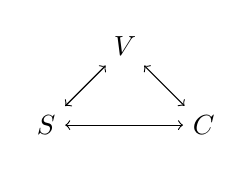
\begin{tikzpicture}
\node (V) at (0,1) {$V$};
\node (S) at (-1,0) {$S$};
\node (C) at (1,0) {$C$};
\draw[<->] (V) to (S);
\draw[<->] (S) to (C);
\draw[<->] (C) to (V);
\end{tikzpicture}}}
\end{equation}
其中 $V$、$S$、$C$ 是 $\SO(8)$ 的八维不可约表示，分别为矢量、旋量和共轭旋量表示。这三个八维不可约表示之间的交换由外自同构诱导，称为群 $\SO(8)$ 的三重性；其 Dynkin 图也画在图 \ref{fig:triality} 中。这一三重性最初由文献 \cite{Seiberg:1994aj} 发现。本小节的论述遵循文献 \cite{Gaiotto:2009we}。

这一系统的希格斯支可以在任一种描述中研究。原来有超多重态 $q_I^a$，其中 $a=1,2$、$I=1,\ldots,8$。规范不变组合为
\begin{equation}
M_{[IJ]}=q_I^aq_J^b\epsilon_{ab}.
\end{equation}
在对偶理论中，有超多重态 $\tilde q^{\tilde a}_{\tilde I}$，其中 $\tilde a=1,2$ 对应对偶 $\SU(2)$，而 $\tilde I=1,\ldots,8$ 对应 $\SO(8)$ 味对称性的旋量表示。此时基本的规范不变量为
\begin{equation}
\tilde M_{[\tilde I\tilde J]}=\tilde q^{\tilde a}_{\tilde I}\tilde q^{\tilde b}_{\tilde J}\epsilon_{\tilde a\tilde b}.
\end{equation}
$M_{[IJ]}$ 和 $\tilde M_{[\tilde I\tilde J]}$ 都处于 $\SO(8)$ 的伴随表示中，可以利用 $\SO(8)$ 的外自同构自然地将它们对应起来。可以检验，$M_{[IJ]}$ 和 $\tilde M_{[\tilde I\tilde J]}$ 满足的约束在外自同构下不变。这表明，希格斯支作为复空间是相同的。
\subsection{推广}\label{sec:trivalent}
\subsubsection{三价图}\index{TrivalentDiagram@三价图|hyperpage}
\begin{figure}[h]
\[
\inc{trivalent}
\]
\caption{三价图及其对应的紫外曲线。\label{fig:trivalent}}
\end{figure}
由 $\cN{=}1$ 手征多重态 $q_{a\alpha u}$（$a,\alpha,u=1,2$）组成的三基本表示超多重态，在迄今的分析中起到了核心作用。我们为它引入一种简记法：如图 \ref{fig:trivalent} 所示，用带有标记 $A$、$B$、$C$ 的三价顶点表示它，分别代表作用于指标 $a$、$\alpha$、$u$ 的对称性 $\SU(2)_A$、$\SU(2)_B$、$\SU(2)_C$。

这一系统的紫外曲线是带有三个穿孔 $A$、$B$、$C$ 的球面，Seiberg-Witten 曲线为
\begin{equation}
\Sigma:\qquad\lambda^2-\phi(z)=0
\end{equation}
其中 $\phi(z)$ 由如下条件确定：在各穿孔 $A,B,C$ 处，二阶极点的系数分别为 $\mu_A^2$、$\mu_B^2$、$\mu_C^2$，如式 \eqref{phicondition_trifund} 所示。

现在，取两个三基本表示超多重态，并将一个 $\SU(2)$ 规范多重态耦合到它们，就可以得到含有四个味的 $\SU(2)$ 理论。我们用两个三价顶点以及连接它们的一条线来表示这一理论，如图 \ref{fig:trivalent} 所示。在连接线上标出指数化耦合 $q$。

从这一三价图出发，很容易写出理论的拉格朗日量。理论的自由参数是质量参数 $\mu_{A,B,C,D}$ 和紫外耦合 $q$。这一系统的紫外曲线是带有四个穿孔 $A$、$B$、$C$、$D$ 的球面，Seiberg-Witten 曲线为
\begin{equation}
\Sigma:\qquad\lambda^2-\phi(z)=0
\end{equation}
其中 $\phi(z)$ 由各穿孔 $X=A,B,C,D$ 处的留数为 $\mu_X^2$ 这一条件确定，如式 \eqref{so8masses} 所示。图 \ref{fig:triality} 已经展示了含有四个味的 $\SU(2)$ 理论的三重性；用三价图可以将其画成图 \ref{fig:triality-trivalent} 的形式。

\begin{figure}[h]
\[
\inc{triality-trivalent}
\]
\caption{用三价图表示的三重性。\label{fig:triality-trivalent}}
\end{figure}

这样，我们可以将三价图视为表示紫外拉格朗日量的简记法。对于给定的这一紫外拉格朗日理论，只需将每个三价顶点替换为一个三穿孔球面，将每条连接线替换为一根连接管，就能得到它的 Seiberg-Witten 解。这是一种出人意料地简洁的、求取 $\cN{=}2$ 规范理论的 Seiberg-Witten 解的方法。

\subsubsection{例：带有一个穿孔的环面}\index{NTwoStarTheory@$\cN{=}2^*$ 理论|hyperpage}\index{WeierstrassFunction@Weierstraß 函数|hyperpage}\index{ModularGroup@模群|hyperpage}
\begin{figure}[h]
\[
\inc{trivalent-n2star}
\]
\caption{含有伴随表示超多重态以及一个自由超多重态的 $\SU(2)$ 理论。\label{fig:n2star}}
\end{figure}
我们来看几个例子。首先，取一个三价顶点，用一条边连接三条线中的两条，见图 \ref{fig:n2star}。我们从由 $\cN{=}1$ 手征多重态 $q_{a\alpha u}$ 描述的三基本表示出发，不过将同一个 $\SU(2)$ 规范多重态耦合到指标 $a$ 和 $\alpha$。于是，组合 $(a,\alpha)$ 处于两个自旋 $1/2$ 表示的张量积中。因此，可以将它分解为一个三重态和一个单态，并带有额外的指标 $u=1,2$：
\begin{equation}
q_{a\alpha u}\to q'_{iu},q''_u,
\end{equation}
其中 $i=1,2,3$ 是 $\SU(2)$ 三重态的指标。

总之，我们只有一个处于三重态中的完整超多重态，以及另一个处于单态中、完全退耦的完整超多重态。因此，这本质上就是 $\cN{=}2^*$ $\SU(2)$ 理论，等价地说，就是对伴随表示超多重态作了质量形变的 $\cN{=}4$ $\SU(2)$ 理论。伴随表示的质量 $\mu$ 与剩下的一个 $\SU(2)$ 味对称性相联系。

用一根管连接三穿孔球面上的两个穿孔，即可得到它的 Seiberg-Witten 解。如图 \ref{fig:n2star} 所示，紫外曲线是带有一个穿孔的环面。此时 Seiberg-Witten 曲线为
\begin{equation}
\lambda^2-\phi(z)=0
\end{equation}
其中 $z$ 现在是环面上的坐标；我们将环面视为施加了等同关系 $z\sim z+1\sim z+\tau$ 的复平面。由于坐标原点可以任意选择，我们将穿孔放在原点。$\phi(z)$ 由如下条件确定：它在 $z=0$ 处有一个给定强度的二阶极点。这一条件将 $\phi(z)$ 的形式唯一确定为
\begin{equation}
\phi(z)=(\mu^2\wp(z;\tau)+u)dz^2
\end{equation}
其中 $\wp$ 是 Weierstra\ss\ 函数，$u$ 是库仑支真空期望值 $u=\vev{\tr\Phi^2}/2$。

现在很清楚，交换单极子与伴随表示夸克之后，耦合由 $\tau$ 给定的理论，与耦合由 $\tau'=-1/\tau$ 给定的同一理论是等价的。耦合空间可以与环面、即亏格为 $1$ 的黎曼曲面的模空间 $\cM_1$ 对应起来，后者为
\begin{equation}
\cM_1=\bH/\SL(2,\bZ)\label{SL2Zfund}
\end{equation}
其中 $\bH$ 是 $\tau$ 取值的上半平面，$\SL(2,\bZ)$ 是交换环面各边的模群。对偶群可以与模群对应起来。

\subsubsection{例：带有五个穿孔的球面}
\begin{figure}[h]
\[
\inc{trivalent-tree}
\]
\caption{一个 $\SU(2)^2$ 理论及其曲线。\label{fig:su2-quiver}}
\end{figure}
再看一个例子：取三个三价顶点，按图 \ref{fig:su2-quiver} 所示的方式将它们连接起来。最左边的三价顶点对于 $\SU(2)_1$ 而言相当于 $N_f=2$ 个味，最右边的三价顶点对于 $\SU(2)_2$ 而言相当于 $N_f=2$ 个味。此外，还有一个来自中央三价顶点的超多重态 $q_{aiu}$，其中 $a$ 对应 $\SU(2)_1$，$i$ 对应 $\SU(2)_2$。剩下的指标 $u=1,2$ 是味对称性的指标。较早的文献更习惯于使用 $\cN{=}1$ 手征多重态 $(Q^i_a,\tilde Q_i^a)$ 来表示这一在 $\SU(2)_1\times\SU(2)_2$ 下带荷的超多重态，其中
\begin{equation}
Q^i_a=q_{aju=1}\epsilon^{ij},\qquad
\tilde Q_i^a=q_{biu=2}\epsilon^{ab}.
\end{equation}
它通常称为在 $\SU(2)_1\times\SU(2)_2$ 下带荷的双基本表示多重态。

这一理论的 Seiberg-Witten 解很容易求得，如图 \ref{fig:su2-quiver} 所示。我们从三个球面出发，分别用复坐标 $z_1$、$z_2$、$z_3$ 描述。穿孔 $A,B$ 位于 $z_1=0,1$；穿孔 $C$ 位于 $z_2=1$；穿孔 $D,E$ 分别位于 $z_3=1,\infty$。为了连接 $z_1=\infty$ 与 $z_2=0$，引入 $w_1=1/z_1$，并要求满足关系 $w_1z_2=q'$。这就意味着有 $z_1=q'z_2$。类似地，连接 $z_2=\infty$ 与 $z_3=0$，就有 $z_2=qz_3$。现在引入 $z=z_3$，用来描述所得到的五穿孔球面上的坐标。于是，各穿孔位于 $z=0$、$qq'$、$q$、$1$ 和 $\infty$，每个穿孔都代表一个 $\SU(2)$ 味对称性，分别记作 $\SU(2)_{A,B,C,D,E}$。$\SU(2)_1\times\SU(2)_2$ 的规范耦合可以与 $q$ 和 $q'$ 对应起来。

将与各味对称性相联系的质量参数记为 $\mu_{A,B,C,D,E}$。Seiberg-Witten 曲线为
\begin{equation}
\lambda^2-\phi(z)=0
\end{equation}
其中 $\phi(z)$ 需要满足渐近行为
\begin{equation}
\phi(z)\sim\frac{\mu_X^2}{z_X^2}dz_X^2\label{massive-full-su2}
\end{equation}
其中，对于 $X=A,B,C,D,E$，$z_X$ 是紫外曲线上的局部坐标，使穿孔 $X$ 位于 $z_X=0$。由 $A$、$B$、$C$、$D$ 处的条件可知，$\phi$ 为
\begin{equation}
\phi(z)=\frac{P(z)}{z^2(z-1)^2(z-q)^2(z-qq')^2}dz^2
\end{equation}
其中 $P(z)$ 是一个多项式。为了施加 $E$ 处的条件，换用坐标 $w=1/z$。要使 $\phi(z)$ 的行为为 $\sim dw^2/w^2$，$P(z)$ 的最高次项只能到 $z^6$。因此，$\phi(z)$ 有七个系数。其中五个组合是质量参数，而不改变二阶极点系数的两个线性组合，则是两个规范多重态 $\SU(2)_{1,2}$ 的库仑支参数 $u=\vev{\tr\Phi^2}/2$ 和 $u'=\vev{\tr\Phi'{}^2}/2$。从 Seiberg-Witten 解可以看出，这一理论具有强弱耦合对偶：只要适当改变两个规范群的耦合 $(q,q')$，就可以任意置换五个味对称群 $\SU(2)_{A,B,C,D,E}$。这一推广的对偶最初由文献 \cite{Argyres:1999fc} 发现。

\subsubsection{例：亏格为二的曲面}\index{MappingClassGroup@映射类群|hyperpage}\index{TeichmullerSpace@Teichmüller 空间|hyperpage}
\begin{figure}[h]
\[
\inc{trivalent-genus2}
\]
\caption{两个 $\SU(2)^3$ 理论及其曲线。\label{fig:genus-2}}
\end{figure}
作为第三个例子，取两个三价顶点，用三条边将它们连接起来。这可以通过两种拓扑上不同的方式实现，如图 \ref{fig:genus-2} 左侧所示。

上方的理论是一个 $\SU(2)_l\times\SU(2)_m\times\SU(2)_r$ 规范理论。它含有处于
\begin{equation}
\mathbf{3}\otimes\mathbf{2}\otimes\mathbf{1},\qquad
\mathbf{1}\otimes\mathbf{2}\otimes\mathbf{3}
\end{equation}
表示中的半超多重态，以及一个在 $\SU(2)_m$ 下带荷的完整超多重态。注意，三价图构造不允许我们考虑最后这个完整超多重态具有非零质量项的理论。下方的理论是一个 $\SU(2)_1\times\SU(2)_2\times\SU(2)_3$ 理论，含有两个三基本表示半超多重态。同样，三价图构造不允许我们为这个三基本表示完整超多重态引入非零质量项。

Seiberg-Witten 解同样很容易得到。为了得到紫外曲线，将两个三价顶点替换为三穿孔球面，再用管将穿孔两两连接起来。可以看到，这两种情形得到的都是光滑的亏格为 $2$ 的曲面。Seiberg-Witten 曲线则是进一步的二重覆盖，由
\begin{equation}
\lambda^2-\phi(z)=0
\end{equation}
给出，其中 $z$ 是亏格为 $2$ 的曲面上的复坐标，$\phi(z)$ 是其上的光滑二次微分。固定亏格为 $2$ 的曲面上的二次微分空间具有三个复维度，我们将它们与库仑支真空期望值 $u_i=\vev{\tr\Phi_i^2}/2$ 对应起来。

现在很清楚，通过调节规范耦合，可以将上方的理论连续地形变为下方的理论。非微扰的耦合空间可以与亏格为 $2$ 的黎曼曲面的模空间 $\cM_2$ 对应起来；该模空间具有三个复维度。对偶群对应于亏格为 $2$ 的曲面的映射类群 $\cG_2$，且 $\cM_2=\cT_2/\cG_2$，其中 $\cT_2$ 是亏格为 $2$ 的黎曼曲面的 Teichm\"uller 空间；可与亏格为 $1$ 的情形式 \eqref{SL2Zfund} 比较。

一个多少有些令人惊讶的数学事实是：$\cT_2$ 在光滑意义下等价于上半平面的三个副本 $\bH^3$，但在全纯意义下并不等价\footnote{作者感谢 Jacques Distler 就这一点所作的极富启发性的讨论。}：
\begin{equation}
\begin{aligned}
\cT_2\simeq\bH^3&\quad\text{在光滑意义下},\\
\cT_2\not\simeq\bH^3&\quad\text{在全纯意义下}.
\end{aligned}
\end{equation}
朴素的微扰分析告诉我们，$\SU(2)^3$ 的耦合空间就是上半平面的三个副本：
\begin{equation}
(\tau_1,\tau_2,\tau_3)\in\bH^3
\end{equation}
而且复结构也包括在内。因此，我们发现，非微扰修正能够使超对称理论参数空间的复结构发生相当剧烈的变化。

\subsubsection{曲线与 Hitchin 场}\label{sec:hitchin}\index{HitchinField@Hitchin 场|hyperpage}\index{HitchinSystem@Hitchin 系统|hyperpage}
我们已经知道，将 Seiberg-Witten 曲线写成
\begin{equation}
\Sigma:\qquad\lambda^2-\phi(z)=0\label{prehitchin}
\end{equation}
的形式，对理解系统很有帮助。曲线的这种表示方式与紫外曲线 $C$ 上所谓的 Hitchin 系统密切相关。对这一技巧的讲解足以另成一份讲义。读者可以从例如文献 \cite{Gaiotto:2009hg} 第 3 节开始了解。

我们至少来非常粗略地介绍它的一个方面。考虑一个无迹的 $2\times2$ 矩阵值亚纯一形式 $\varphi(z)$。于是，可以对一形式 $\lambda$ 构造如下形式的方程：
% [Tutor Note: p.105 原文 "We consider a meromoprhic one-form $\varphi(z)$" 中 "meromoprhic" 应为 "meromorphic"，系拼写笔误；译文按其本意作“亚纯一形式”。]
\begin{equation}
\det(\lambda-\varphi(z))=0.\label{hitchin}
\end{equation}
将式 \eqref{prehitchin} 与式 \eqref{hitchin} 对应起来，得到
\begin{equation}
\frac12\tr\varphi(z)^2=\phi(z).\label{p-p}
\end{equation}
这一矩阵场 $\varphi(z)$ 称为 Hitchin 场\footnote{Hitchin 本人将 $\varphi(z)$ 称为希格斯场，但作者认为，在 $\cN{=}2$ 超对称语境中，这一术语颇易引起混淆，因为 $\varphi(z)$ 控制的是库仑支的物理，而不是希格斯支的物理。}。可以利用弦对偶来理解为何紫外曲线上存在这样一个复的伴随表示场，不过对它的解释超出了本讲义的目的。

在与质量项 $\mu_X$ 相联系、位于 $z_X=0$ 的穿孔处，场 $\phi(z)$ 的条件已在式 \eqref{massive-full-su2} 中给出：
\begin{equation}
\phi(z)=\mu_X^2\frac{dz_X^2}{z_X^2}+\text{（奇异性较弱的项）}.\label{phi-full}
\end{equation}
它转化为 Hitchin 场 $\varphi(z)$ 的条件
\begin{equation}
\varphi(z)\sim\begin{pmatrix}
\mu_X&0\\
0&-\mu_X
\end{pmatrix}\frac{dz_X}{z_X}+\text{（奇异性较弱的项）}.\label{varphi-full}
\end{equation}
这里，符号 $A\sim B$ 表示 $A$ 与 $B$ 共轭，也就是说，存在可逆的 $N\times N$ 复矩阵 $g$，使得 $A=gBg^{-1}$。

现在，考虑将 $\mu_X$ 关掉、令其为零时会发生什么。在式 \eqref{phi-full} 的描述中，边界条件变为
\begin{equation}
\phi(z)=c\frac{dz_X^2}{z_X}+\text{（奇异性较弱的项）}\label{q-q}
\end{equation}
其中 $c$ 是某个常数。而在式 \eqref{varphi-full} 的描述中，留数并不是简单地变成零矩阵。注意，只要 $\mu_X\neq0$，就有
\begin{equation}
\begin{pmatrix}
\mu_X&0\\
0&-\mu_X
\end{pmatrix}
\sim
\begin{pmatrix}
\mu_X&1\\
0&-\mu_X
\end{pmatrix},
\end{equation}
而且可以在右侧取极限 $\mu_X\to0$。这意味着，无质量极限给出的边界条件具有如下形式：
\begin{equation}
\varphi(z)\sim\begin{pmatrix}
0&1\\
0&0
\end{pmatrix}\frac{dz_X}{z_X}+\text{（奇异性较弱的项）}.
\end{equation}
利用式 \eqref{p-p}，可以发现它重现了条件 \eqref{q-q}。

在这一阶段，使用 $\varphi(z)$ 而不是 $\phi(z)$ 的优点可能还不太明显。然而，当我们讨论推广到 $\SU(N)$ 规范理论，或具有更复杂规范群的规范理论时，它就会变得至关重要。
% [Tutor Note: p.106 原文 "one might not find the advantange of using $\varphi(z)$ instead of $\phi(z)$ very much" 中 "advantange" 应为 "advantage"；同段 "It turns out, however, that … it turns out to be crucial" 重复了 "turns out"。两处均为笔误，译文按本意译出。]

\subsection{再论味数较少的理论}\label{sec:less}\index{WildPuncture@野性穿孔|hyperpage}
我们发现，将 $N_f=4$ 理论的 Seiberg-Witten 曲线写成
\begin{equation}
\lambda^2-\phi(z)=0
\end{equation}
的形式，极大地有助于理解对偶的结构。现在将这一思想应用于味数较少、即 $N_f<4$ 的理论的曲线。

\subsubsection{曲线的改写}
首先，考虑纯理论的曲线，
\begin{equation}
\frac{\Lambda^2}z+\Lambda^2z=x^2-u,\qquad\text{其中}\ \lambda=x\frac{dz}z.
\end{equation}
用 $\lambda$ 可以将它写成
\begin{equation}
\lambda^2-\phi(z)=0,\qquad\phi(z)=(\frac{\Lambda^2}z+u+\Lambda^2z)\frac{dz^2}{z^2}.
\end{equation}
可以看到，二次微分 $\phi(z)$ 的奇异性比 $N_f=4$ 理论中的更强：现在它在 $z=0$ 和 $=\infty$ 处具有三阶极点。曲线的情形可以画成图 \ref{fig:lessG} 上排的样子。其中，罗马数字 III 表示 $\phi(z)$ 在该穿孔处具有三阶极点。$\phi(z)$ 的高阶极点奇异性构成了一类新的穿孔，我们将它们称为野性 $\SU(2)$ 穿孔。

作为编码紫外拉格朗日量的三价图的推广，我们引入如下记号：一条边代表一个 $\cN{=}2$ $\SU(2)$ 矢量多重态，而一端的黑色方块表示不引入任何超多重态。于是，很容易看出从表示紫外拉格朗日量的图到紫外曲线的转换关系，如图 \ref{fig:lessG} 所示。
\begin{figure}[h]
\[
\inc{trivalent-lessflavorsXX}
\]
\caption{味数较少的 $\SU(2)$ 理论。\label{fig:lessG}}
\end{figure}
其次，考虑 $N_f=1$ 理论的曲线，
\begin{equation}
\frac{2\Lambda(\tilde x-\mu)}z+\Lambda^2z=\tilde x^2-u,\qquad\text{其中}\ \tilde\lambda=\tilde x\frac{dz}z.
\end{equation}
它可以写成
\begin{equation}
\lambda^2-\phi(z)=0,\qquad\phi(z)=(\frac{\Lambda^2}{z^2}-\frac{2\Lambda\mu}z+u+\Lambda^2z)\frac{dz^2}{z^2}
\end{equation}
其中 $\lambda=xdz/z$ 由 $\tilde\lambda$ 平移而来。我们发现，$z=0$ 处的奇点变成了四阶极点。拉格朗日量及其 Seiberg-Witten 解可以简洁地概括为图 \ref{fig:lessG} 下排的形式。边代表一个 $\SU(2)$ 规范群。一端的黑色方块表示那里没有任何超多重态。另一端的浅色圆点表示引入一个二重态超多重态。将黑色方块对应于一个带有三阶极点、用 III 标记的球面，类似地将浅色圆点对应于一个带有四阶极点、用 IV 标记的球面，最后用一根管将它们连接起来，即可得到解。注意，四阶极点具有自己的 $\SU(2)$ 味对称性和相应的质量参数。

总之，我们将带有一个正则穿孔和一个极点阶数为 III 的野性穿孔的球面视为空理论，将带有一个正则穿孔和一个极点阶数为 IV 的野性穿孔的球面视为退耦的二重态超多重态理论，如图 \ref{fig:lessG} 所示。用管连接正则穿孔，就得到味数较少的理论的紫外曲线。

\subsubsection{推广}
\begin{figure}[h]
\[
\inc{trivalent-mixedX}
\]
\caption{一个 $\SU(2)^4$ 理论及其曲线。\label{fig:complicated-example}}
\end{figure}
这一推广使我们能够求出一大类 $\cN{=}2$ 理论的 Seiberg-Witten 解，其规范群是若干个 $\SU(2)$ 的乘积。例如，考虑图 \ref{fig:complicated-example} 左侧描述的、规范群为 $\SU(2)^4$ 的紫外拉格朗日理论。用文字来说，我们先取三个双基本表示超多重态，
\begin{equation}
Q_{aiu},\quad Q'_{us\alpha},\quad Q''_{\alpha xm}.
\end{equation}
图中展示了如何将各指标分配到三价图的边上。对应于动力学规范群的边用粗线突出表示。用文字来说，指标 $a,i,m$ 对应于 $\SU(2)_{A,B,C}$ 味对称性。一个 $\SU(2)$ 规范多重态耦合到指标 $u$，指数化耦合常数为 $q$；另一个 $\SU(2)$ 规范多重态耦合到指标 $\alpha$，指数化耦合常数为 $q'$。再引入一个 $\SU(2)_1$ 规范多重态，使其耦合到黑色方块所对应的指标 $s$；最后再引入一个 $\SU(2)_2$ 规范多重态，使其耦合到指标 $x$，并额外带有 $N_f=1$ 个超多重态 $(Q''''{}_x,\tilde Q''''{}^x)$。必要时我们可以写出拉格朗日量，但现在已经可以看出，三价图对其结构的概括是多么简洁。

它的 Seiberg-Witten 解可以立即得到，由
\begin{equation}
\lambda^2-\phi(z)=0,
\end{equation}
给出，其中 $\phi(z)$ 有三个二阶极点、一个三阶极点，以及一个四阶极点。分别将它们放在 $z=0,1,z_0$、$z_1$ 和 $\infty$ 处，可以看到 $\phi(z)$ 具有形式
\begin{equation}
\phi(z)=\frac{P(z)}{z^2(z-1)^2(z-z_0)^2(z-z_1)^3}dz^2
\end{equation}
其中 $P(z)$ 是一个多项式。要在 $w=1/z=0$ 处具有四阶极点，$P(z)$ 必须是九次多项式。在十个系数中，三个是 $\SU(2)_{A,B,C}$ 味对称性的质量参数，一个是黑色圆点所对应的 $\SU(2)_1$ 的能标，一个是 $\SU(2)_2$ 的能标，还有一个是 $\SU(2)_2$ 的额外 $N_f=1$ 个味的质量参数。剩下的四个线性组合可以与四个库仑支参数 $u_i=\vev{\tr\Phi_i^2/2}$ 对应起来。这不是一个共形理论：它具有两个动力学能标 $\Lambda$ 和 $\Lambda'$。尽管如此，从紫外曲线的结构仍然可以立即看出，存在交换 $A$、$B$、$C$ 处三个正则穿孔的 S 对偶。
